\documentclass[aspectratio=169,11pt]{beamer}

\usepackage{iftex}
\ifXeTeX
  \usepackage{fontspec}
  \usepackage{xeCJK}
  \setmainfont{Times New Roman}
  \IfFontExistsTF{Microsoft JhengHei}{
    \setCJKmainfont{Microsoft JhengHei}
    \setCJKsansfont{Microsoft JhengHei}
    \setCJKmonofont{Microsoft JhengHei}
  }{
    \setCJKmainfont{SimSun}
    \setCJKsansfont{SimSun}
    \setCJKmonofont{SimSun}
  }
  \IfFontExistsTF{Consolas}{\setmonofont{Consolas}}{}
\fi
\usepackage{amsmath}
\usepackage{array}
\usepackage{booktabs}
\usepackage{graphicx}
\usepackage{siunitx}
\usepackage{xcolor}
\usepackage{xurl}

\usetheme{Madrid}
\usecolortheme{default}
\setbeamertemplate{navigation symbols}{}
\setbeamertemplate{footline}[frame number]
\graphicspath{{assets/}}
\urlstyle{same}

\definecolor{goodGreen}{RGB}{35,120,75}
\definecolor{warnRed}{RGB}{170,55,55}
\definecolor{aaltoBlue}{RGB}{0,83,155}

\newcommand{\good}[1]{\textcolor{goodGreen}{#1}}
\newcommand{\warn}[1]{\textcolor{warnRed}{#1}}
\newcommand{\blue}[1]{\textcolor{aaltoBlue}{#1}}
\newcommand{\src}[1]{\vfill{\tiny\textcolor{gray!70!black}{Source: \url{#1}}}}
\newcommand{\pathtext}[1]{{\scriptsize\url{#1}}}
\newcolumntype{L}[1]{>{\raggedright\arraybackslash}p{#1}}
\newcolumntype{R}[1]{>{\raggedleft\arraybackslash}p{#1}}

\title[Baseline Comparison]{物理基线、Production MLP 与 SVGP 对比}
\subtitle{2026-05-21 full-clean / uncensored CDF / P50--Q1 统一评估}
\author{Linan Jiang}
\institute{Aalto University}
\date{21 May 2026}

\begin{document}

\begin{frame}
  \titlepage
\end{frame}

\begin{frame}{为什么更新这组 slides}
\small
\begin{block}{旧版本的问题}
旧 baseline deck 主要记录 5 月上旬的中间模型，且叙事重点是 MLP 相对早期
GP baseline 的提升。
\end{block}

\begin{block}{现在的论文口径}
最新比较使用同一批 2026-05-21 评估产物：production MLP 五 seed、
mu-anchor/raw-uncertain 变体、Stage-3 SVGP、以及重新拟合的
Hiroyasu--Arai / Naber--Siebers。
\end{block}

\begin{block}{一句话结论}
\good{Production MLP 显著优于 HA/NS 物理曲线基线；SVGP 在点预测 RMSE/MAE
上仍略领先；MLP 的优势是更保守的不确定度覆盖，适合作为 screening surrogate。}
\end{block}
\end{frame}

\begin{frame}{评估协议}
\small
\begin{tabular}{L{0.26\linewidth}R{0.17\linewidth}R{0.18\linewidth}L{0.31\linewidth}}
\toprule
口径 & 点数 & 工况/轨迹 & 作用 \\
\midrule
Full-clean CDF & \num{692942} & \num{24316} trajectories & 主 headline；所有模型在同一 clean CDF 点集上比较。 \\
Conservative uncensored CDF & \num{542565} & 592 conditions & 排除保守判定的 FOV 右删失和信号衰减时间桶。 \\
P50 observed & \num{4213} & 495 conditions & 按工况聚合后的 P50 观测点，检验均值头的稳健性。 \\
Q1 extrapolated grid & \num{21527} & 495 conditions & P50/Q1 拟合外推区间；主要看 mu 头的外推趋势。 \\
\bottomrule
\end{tabular}

\vspace{0.6em}
\footnotesize
这些口径不是互相替代：full-clean 给整体 CDF 精度，uncensored CDF 控制删失偏差，
P50/Q1 检查按工况压缩之后的稳健性和外推行为。
\src{Thesis/generated/baseline_comparison_20260521/summary.json}
\end{frame}

\begin{frame}{模型组}
\small
\begin{tabular}{L{0.30\linewidth}L{0.58\linewidth}}
\toprule
模型 & 设置 \\
\midrule
Hiroyasu--Arai calibrated & 在当前 clean 口径重新校准的经验曲线基线。 \\
Naber--Siebers delay & 带 delay 处理的经验曲线基线，同样重新拟合。 \\
Production MLP & Stage-3 \texttt{anchor\_off}，seeds 7/17/42/99/2024，报告 mean \(\pm\) std。 \\
mu-anchor raw-uncertain prodKD & 同数据、同 teacher 热启动的 mu-anchor/raw-uncertain/product KD 组合。 \\
Stage-3 SVGP & 稀疏异方差 GP baseline，seed 42，吃同一 full-clean / fixed-table 评估数据。 \\
\bottomrule
\end{tabular}

\vspace{0.7em}
\begin{block}{公平比较边界}
\footnotesize
这里比较的是同数据评估口径，不把 production 模型直接和 LONO 结果混读。
LONO 是泛化压力测试，已经拆到独立 stage-1/2/3 ablation decks。
\end{block}
\end{frame}

\begin{frame}{Full-Clean Headline}
\scriptsize
\begin{tabular}{L{0.29\linewidth}R{0.10\linewidth}R{0.10\linewidth}R{0.10\linewidth}R{0.10\linewidth}R{0.10\linewidth}R{0.10\linewidth}}
\toprule
模型 & RMSE & MAE & Bias & P95 & Cov1 & Cov2 \\
\midrule
Hiroyasu--Arai & 11.268 & 8.658 & +0.288 & 22.891 & 0.615 & 0.912 \\
Naber--Siebers & 10.545 & 8.177 & -0.442 & 21.253 & 0.637 & 0.919 \\
\good{Production MLP mean(5)} & \good{4.735} & \good{3.293} & +0.626 & \good{9.167} & \good{0.867} & \good{0.985} \\
mu-anchor raw-uncertain & 5.200 & 3.654 & -0.585 & 10.525 & 0.834 & 0.985 \\
\blue{SVGP Stage-3} & \blue{4.628} & \blue{3.173} & -0.070 & 9.242 & 0.703 & 0.939 \\
\bottomrule
\end{tabular}

\vspace{0.6em}
\small
Production MLP 比 HA/NS 降低超过一半 RMSE，但 SVGP 仍是 full-clean 点预测
精度冠军。MLP 的 1\(\sigma\)/2\(\sigma\) coverage 明显更保守。
\src{Thesis/generated/baseline_comparison_20260521/headline_full_clean.csv}
\end{frame}

\begin{frame}{Full-Clean: Error Metrics}
\centering
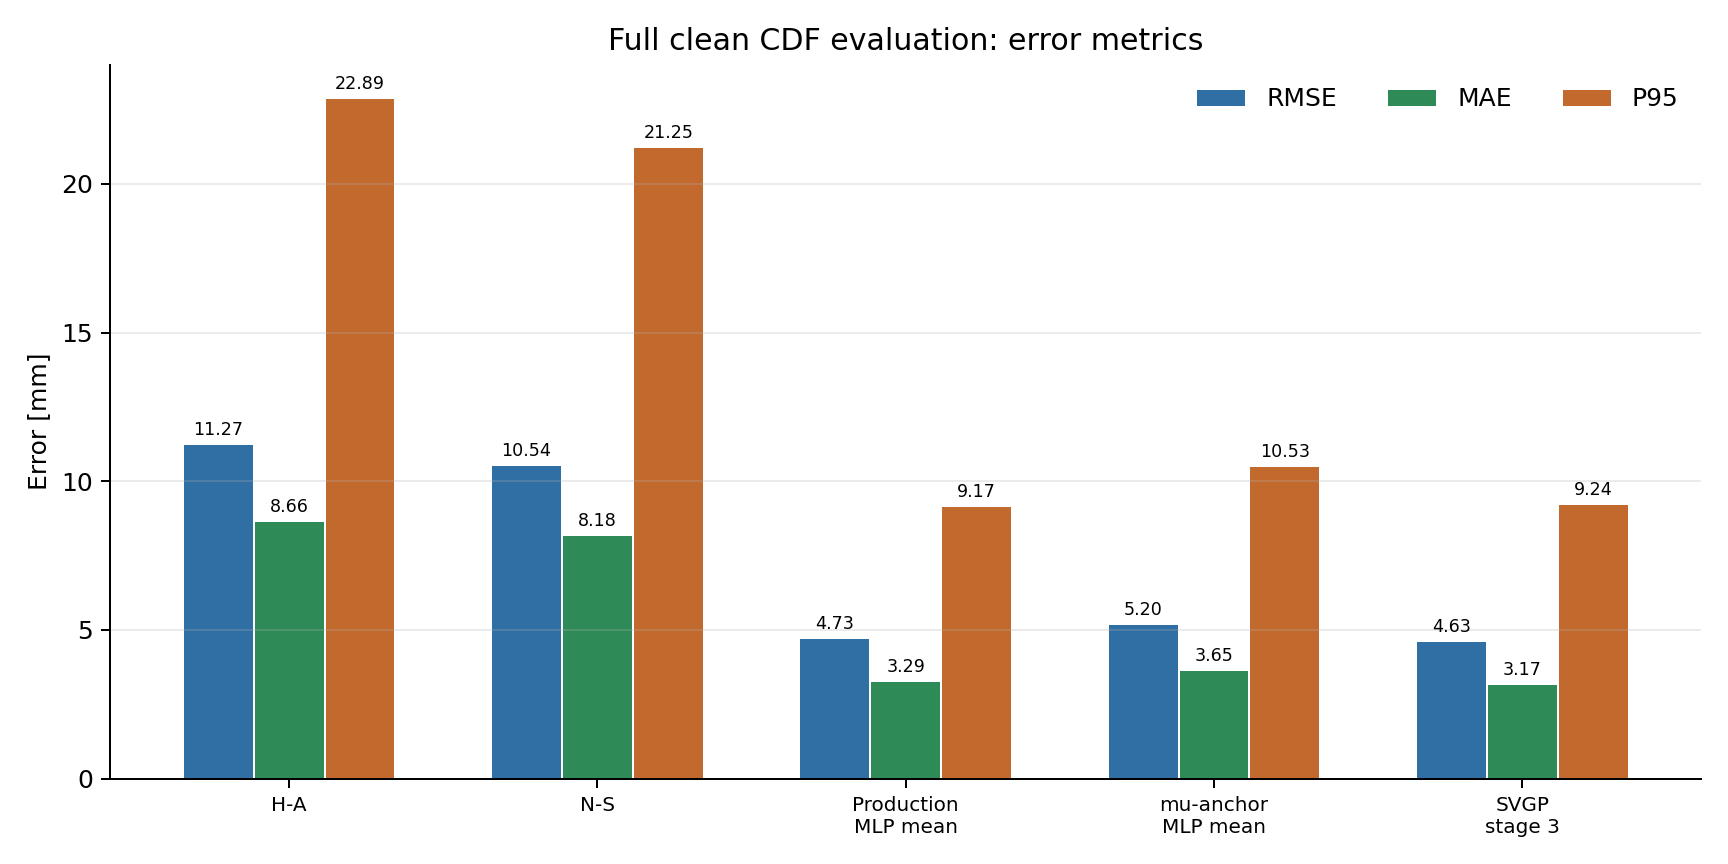
\includegraphics[width=0.92\linewidth,height=0.74\textheight,keepaspectratio]{full_clean_metric_bars_rmse_mae_p95.png}
\src{Thesis/images/baseline_comparison_20260521/full_clean_metric_bars_rmse_mae_p95.png}
\end{frame}

\begin{frame}{Full-Clean: Coverage}
\centering
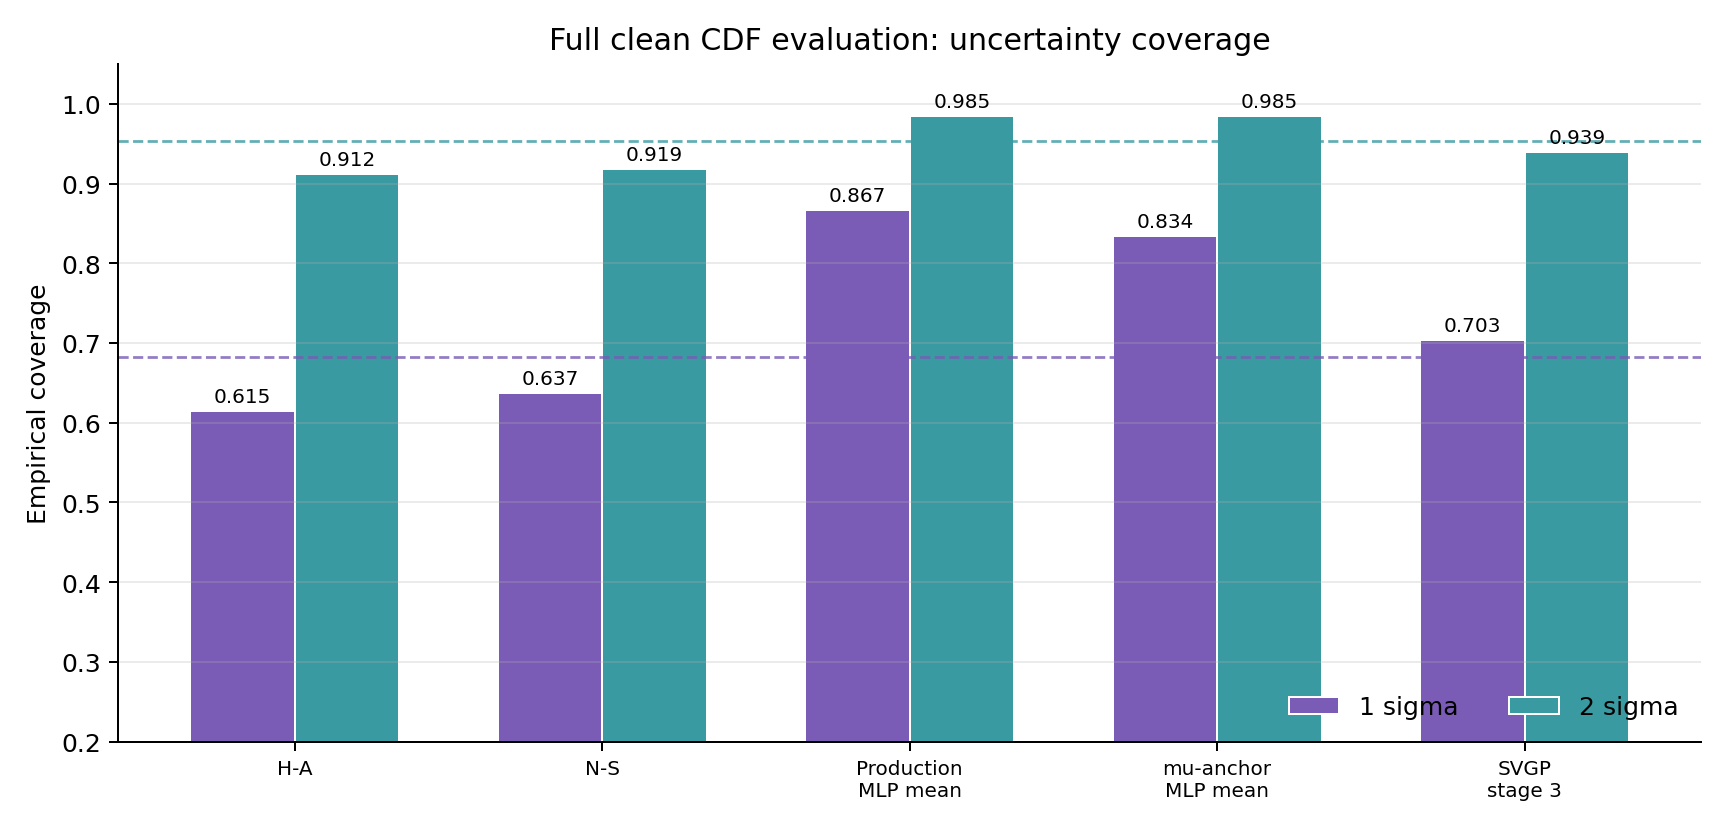
\includegraphics[width=0.88\linewidth,height=0.74\textheight,keepaspectratio]{full_clean_coverage_comparison.png}
\src{Thesis/images/baseline_comparison_20260521/full_clean_coverage_comparison.png}
\end{frame}

\begin{frame}{Production MLP 五 seed 稳定性}
\begin{columns}[T,onlytextwidth]
\begin{column}{0.58\linewidth}
\centering
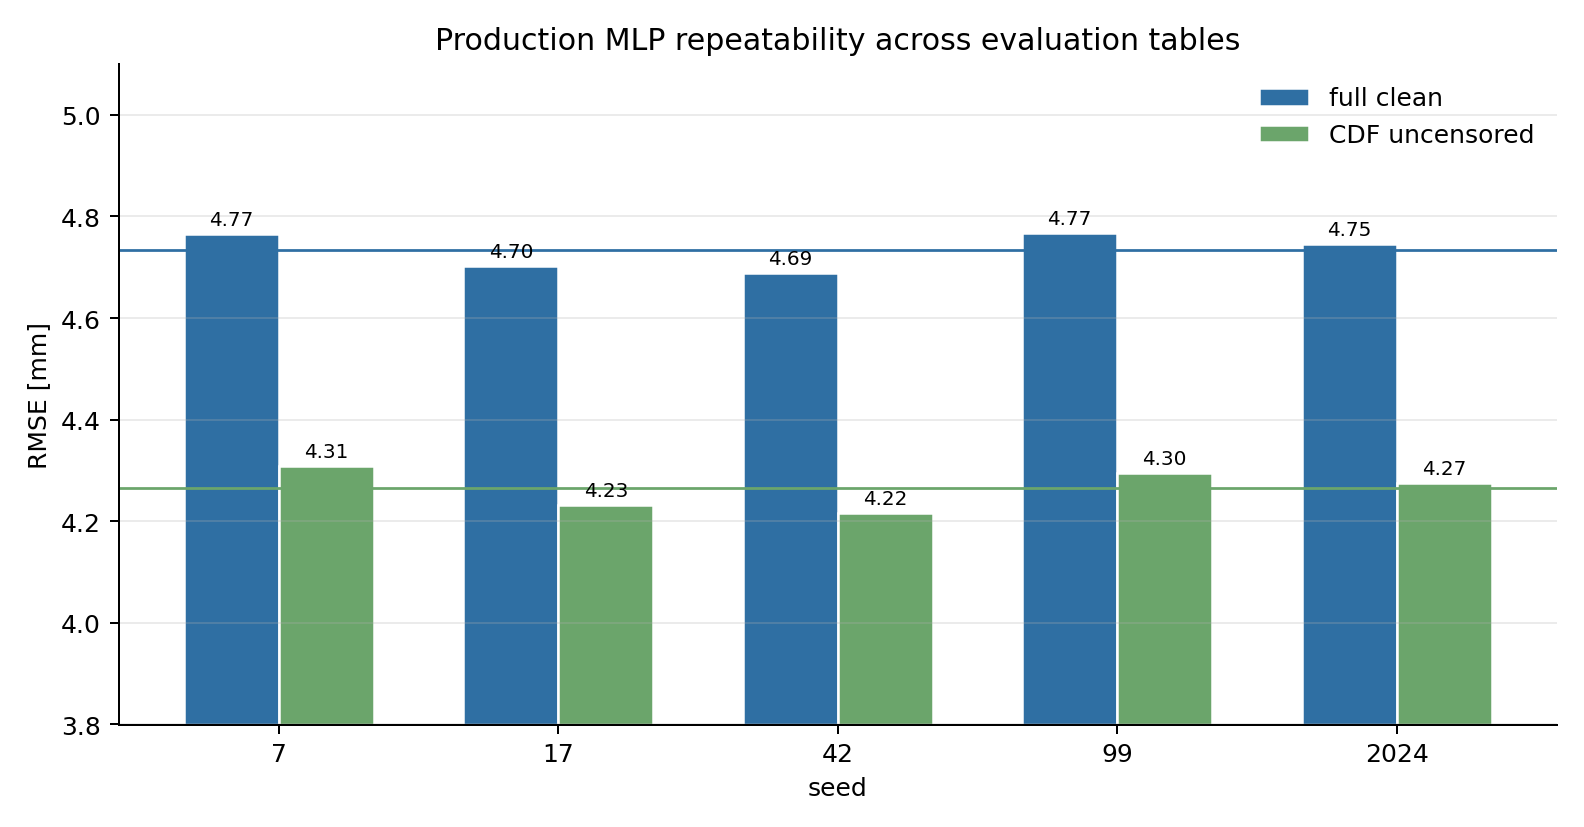
\includegraphics[width=\linewidth,height=0.70\textheight,keepaspectratio]{production_mlp_per_seed_rmse.png}
\end{column}
\begin{column}{0.38\linewidth}
\small
\begin{block}{Full-clean aggregate}
\begin{itemize}
  \item RMSE \(= \SI{4.735}{mm} \pm \SI{0.037}{mm}\)
  \item MAE \(= \SI{3.293}{mm} \pm \SI{0.039}{mm}\)
  \item Bias \(= +\SI{0.626}{mm} \pm \SI{0.112}{mm}\)
  \item Cov1/Cov2 \(= 0.867 / 0.985\)
\end{itemize}
\end{block}
\begin{block}{读法}
\footnotesize
这不是 seed luck：五个 seed 的 RMSE spread 只有约 \SI{0.04}{mm}。
\end{block}
\end{column}
\end{columns}
\src{Thesis/generated/baseline_comparison_20260521/production_mlp_full_clean_per_seed.csv}
\end{frame}

\begin{frame}{Conservative Uncensored CDF}
\scriptsize
\begin{tabular}{L{0.29\linewidth}R{0.10\linewidth}R{0.10\linewidth}R{0.10\linewidth}R{0.10\linewidth}R{0.10\linewidth}R{0.10\linewidth}}
\toprule
模型 & RMSE & MAE & Bias & P95 & Cov1 & Cov2 \\
\midrule
Hiroyasu--Arai & 10.261 & 7.767 & +2.152 & 21.095 & 0.630 & 0.917 \\
Naber--Siebers & 9.286 & 7.195 & +0.628 & 18.408 & 0.659 & 0.927 \\
\good{Production MLP mean(5)} & \good{4.265} & \good{3.032} & +0.562 & \good{8.307} & \good{0.887} & \good{0.989} \\
mu-anchor raw-uncertain & 4.941 & 3.505 & -0.868 & 10.123 & 0.840 & 0.988 \\
\blue{SVGP Stage-3} & \blue{4.193} & \blue{2.894} & -0.040 & 8.461 & 0.716 & 0.945 \\
\bottomrule
\end{tabular}

\vspace{0.6em}
\small
删失保守过滤后，production MLP 和 SVGP 的点误差仍非常接近；SVGP RMSE
略低，MLP coverage 更宽。
\src{Thesis/generated/baseline_comparison_20260521/fixed_table_group_summary.csv}
\end{frame}

\begin{frame}{Uncensored CDF: Error and Coverage}
\begin{columns}[T,onlytextwidth]
\begin{column}{0.50\linewidth}
\centering
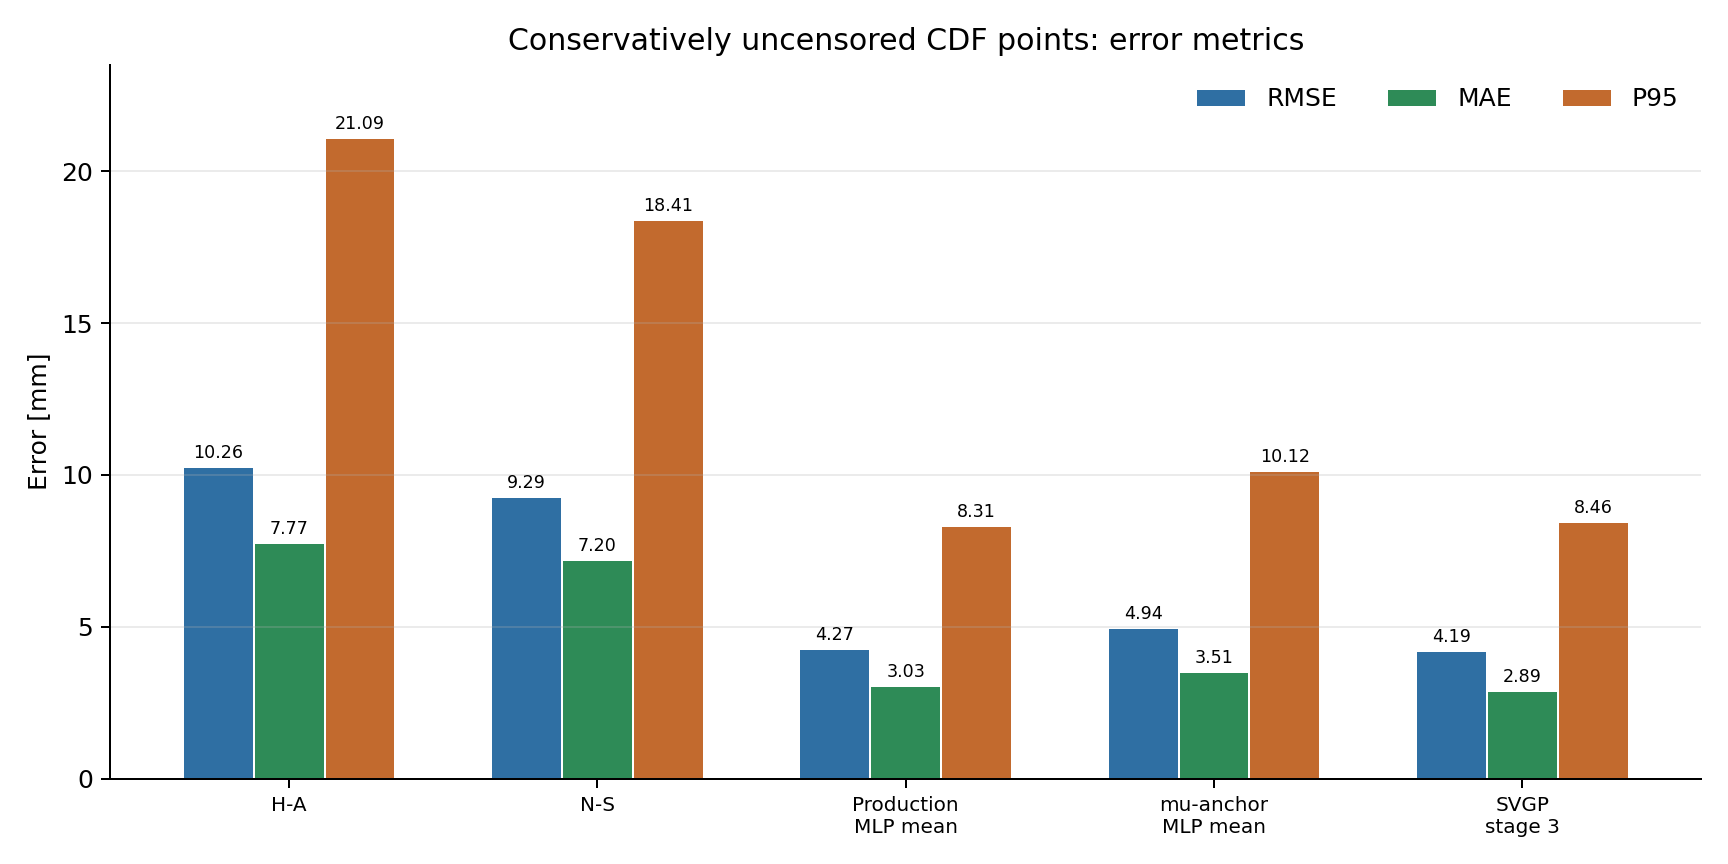
\includegraphics[width=\linewidth,height=0.70\textheight,keepaspectratio]{cdf_uncensored_metric_bars_rmse_mae_p95.png}
\end{column}
\begin{column}{0.50\linewidth}
\centering
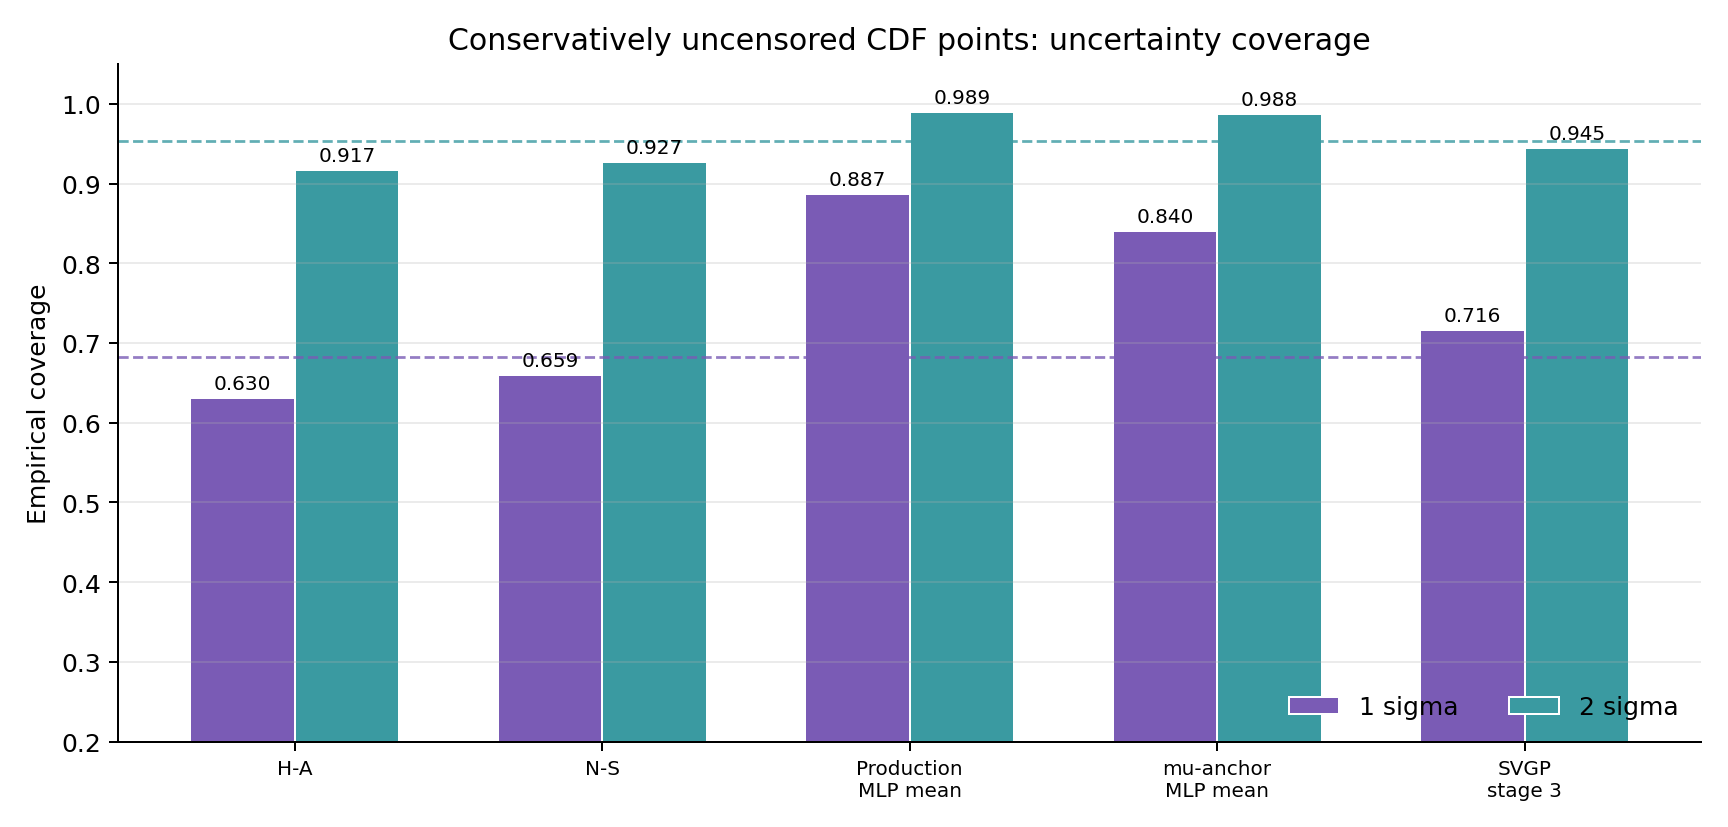
\includegraphics[width=\linewidth,height=0.70\textheight,keepaspectratio]{cdf_uncensored_coverage_comparison.png}
\end{column}
\end{columns}
\src{Thesis/images/baseline_comparison_20260521/cdf_uncensored_*.png}
\end{frame}

\begin{frame}{P50 与 Q1 口径}
\scriptsize
\begin{tabular}{L{0.27\linewidth}R{0.13\linewidth}R{0.13\linewidth}R{0.13\linewidth}R{0.13\linewidth}}
\toprule
模型 & P50 RMSE & P50 MAE & Q1 extrap. RMSE & Q1 extrap. MAE \\
\midrule
Q1 oracle & 1.010 & 0.689 & -- & -- \\
Hiroyasu--Arai & 9.948 & 7.662 & 31.837 & 25.316 \\
Naber--Siebers & 9.048 & 7.206 & 39.818 & 32.216 \\
\good{Production MLP mean(5)} & \good{2.848} & \good{1.826} & 10.864 & 7.380 \\
\good{mu-anchor raw-uncertain} & 3.212 & 2.147 & \good{10.358} & \good{6.965} \\
\blue{SVGP Stage-3} & \blue{2.649} & \blue{1.603} & 10.591 & 7.236 \\
\bottomrule
\end{tabular}

\vspace{0.6em}
\small
P50 observed 上 SVGP 最好；Q1 extrapolated 上 mu-anchor 组合略有帮助，
但这不是 full-clean 主模型的胜利，只说明 mu 头对外推网格有局部价值。
\src{Thesis/generated/baseline_comparison_20260521/fixed_table_group_summary.csv}
\end{frame}

\begin{frame}{P50 Observed 与 Q1 Extrapolated}
\begin{columns}[T,onlytextwidth]
\begin{column}{0.50\linewidth}
\centering
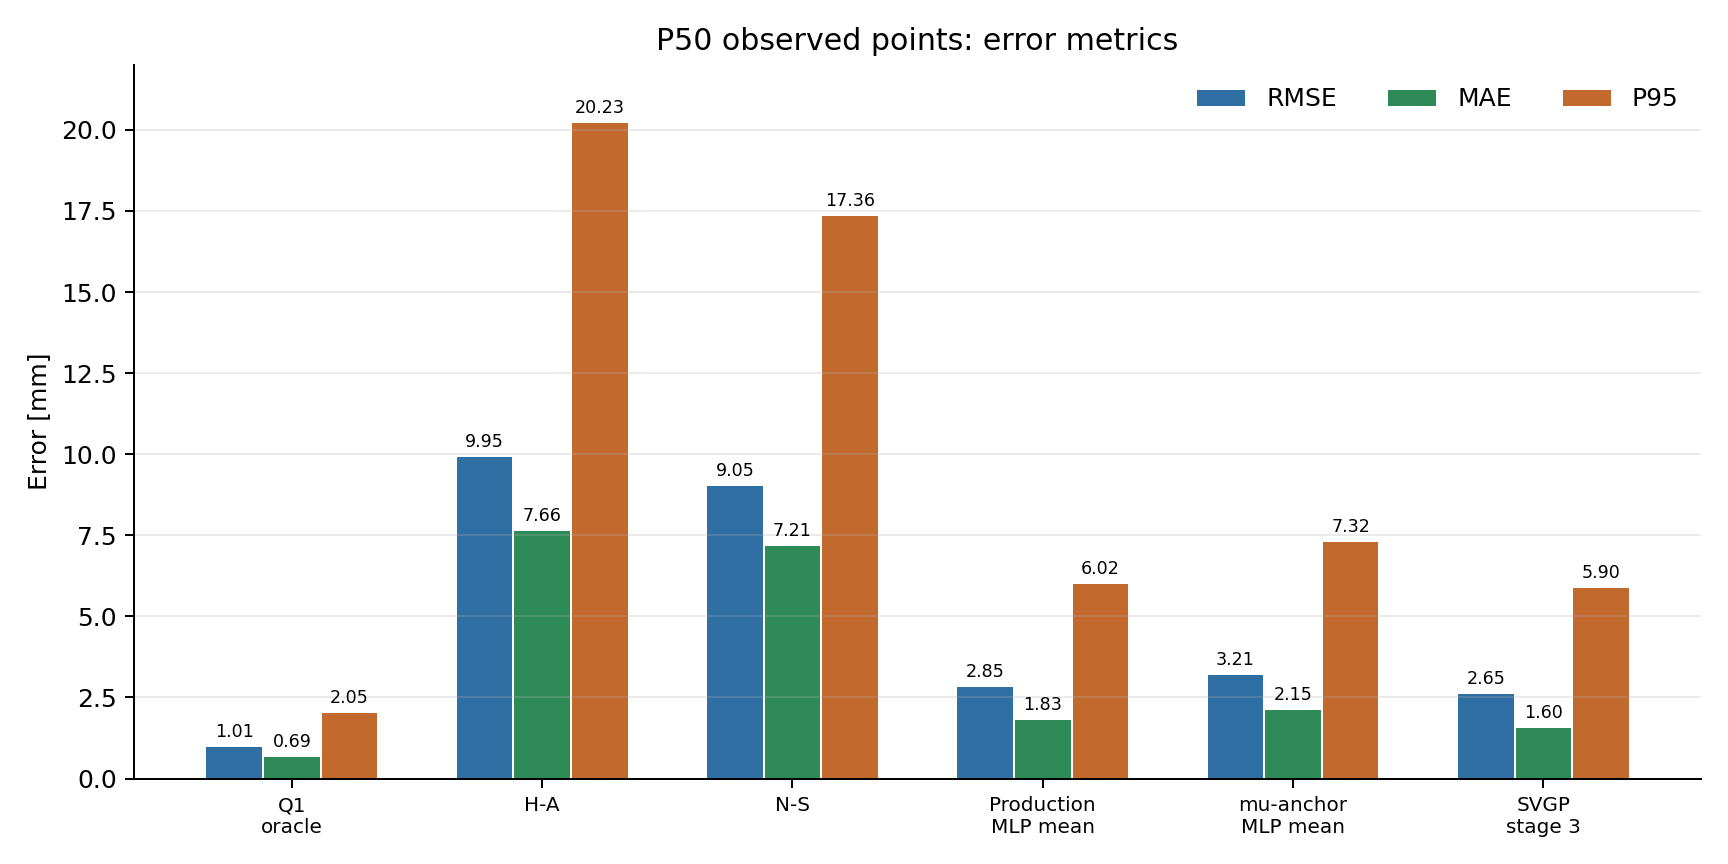
\includegraphics[width=\linewidth,height=0.70\textheight,keepaspectratio]{p50_observed_metric_bars_rmse_mae_p95.png}
\end{column}
\begin{column}{0.50\linewidth}
\centering
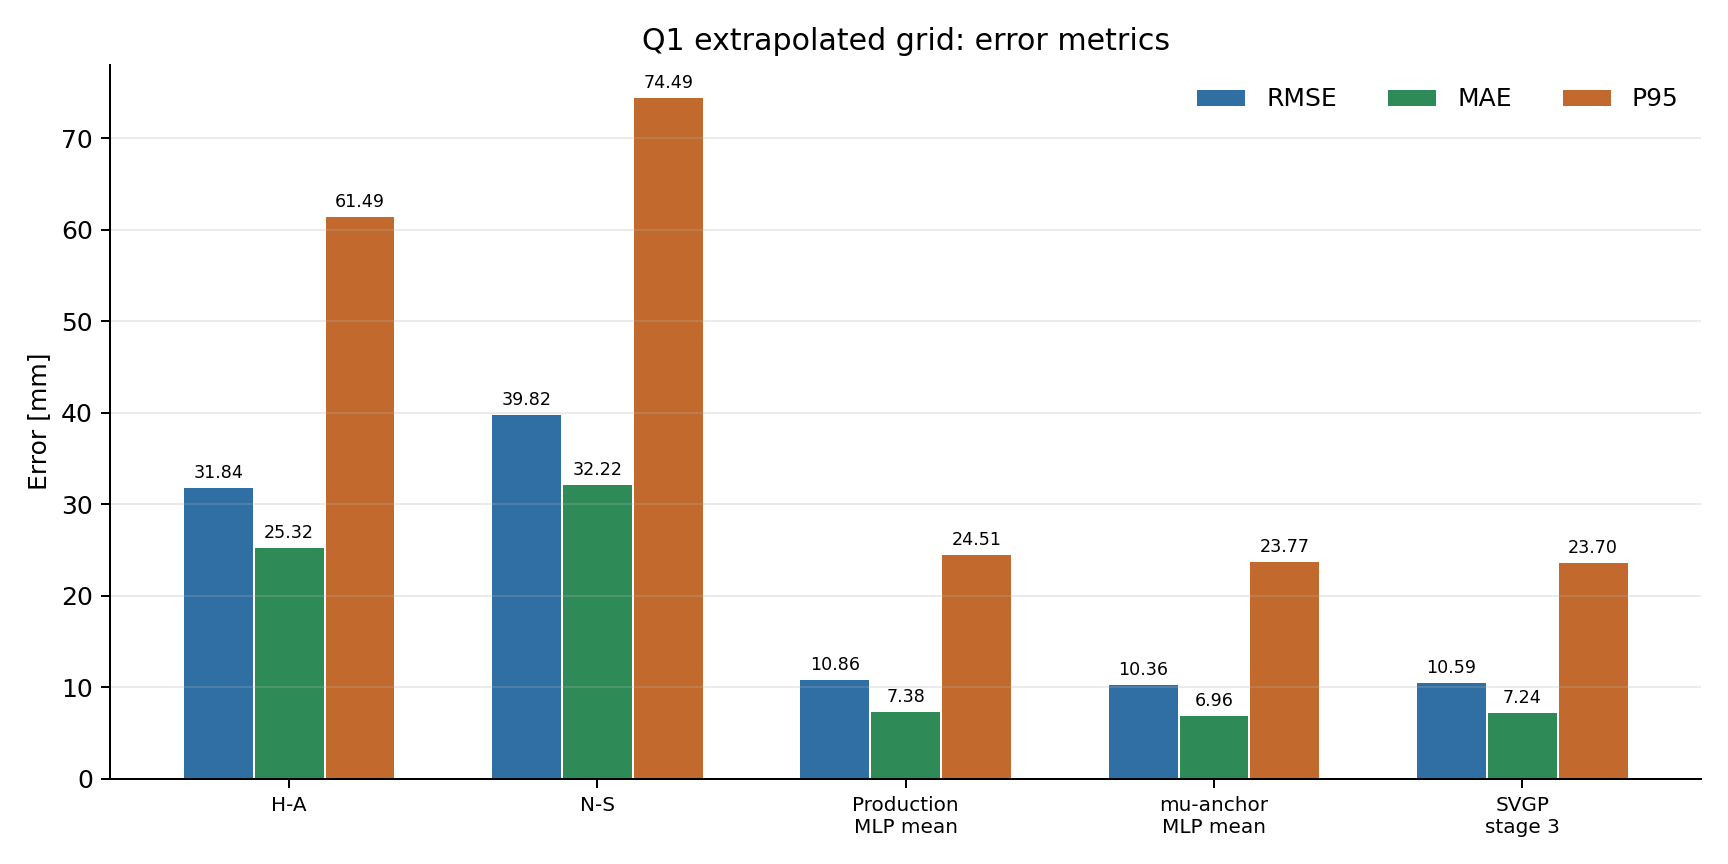
\includegraphics[width=\linewidth,height=0.70\textheight,keepaspectratio]{q1_extrapolated_metric_bars_rmse_mae_p95.png}
\end{column}
\end{columns}
\src{Thesis/images/baseline_comparison_20260521/p50_observed_*.png; q1_extrapolated_*.png}
\end{frame}

\begin{frame}{论文叙事建议}
\small
\begin{enumerate}
  \item 不说 MLP 已经超过 SVGP；最新实验证据不支持这个强表述。
  \item 可以说 production MLP 在所有 clean / uncensored / P50 口径下都远强于 HA/NS。
  \item 可以说 SVGP 在点预测上略优，尤其 RMSE/MAE；这是公平的 ML baseline。
  \item 可以强调 MLP 的 coverage 更保守，适合 downstream screening 和安全余量估计。
  \item 可以把 mu-anchor/raw-uncertain 放到 Q1 extrapolation 的补充结果里，而不是主 headline。
\end{enumerate}
\end{frame}

\begin{frame}{文件索引}
\small
\begin{tabular}{L{0.30\linewidth}L{0.60\linewidth}}
\toprule
内容 & 路径 \\
\midrule
Slides source & \pathtext{Thesis/slides/baseline_comparison_slides_zh/baseline_comparison_slides_zh.tex} \\
Figures & \pathtext{Thesis/images/baseline_comparison_20260521/} \\
Generated tables & \pathtext{Thesis/generated/baseline_comparison_20260521/} \\
Fixed-table report & \pathtext{MLP/baseline/comparison_reports/stage3_fixed_table_eval_with_ha_ns_20260521/} \\
Full-clean MLP vs SVGP & \pathtext{MLP/baseline/comparison_reports/mlp_production_stage3_vs_svgp_stage3_full_clean_20260521/} \\
Figure script & \pathtext{Thesis/generated/baseline_comparison_20260521/make_figures.py} \\
\bottomrule
\end{tabular}
\end{frame}

\end{document}
